% % part: 支持向量机
% % chapter: 中级支持向量机

% \documentclass[UTF8]{ctexbook}

% \ctexset{
%     part/number = \chinese{part}
% }
% \usepackage{multirow}
% \usepackage{amsmath}% ams 数学公式
% \usepackage{amsfonts}% ams 数学字体
% \usepackage{bbm}%重影字体
% \usepackage{amssymb,latexsym}% ams 数学符号与LaTeX数学符号
% \usepackage{mathrsfs}% 花式符号
% \usepackage{ntheorem}%定理、定义、证明
%     \theoremstyle{nonumberplain}
%     \theoremheaderfont{\bfseries}
%     \theorembodyfont{\normalfont}
%     \theoremsymbol{$\square$}
%     \newtheorem{Proof}{\hskip 2em 证明}
%     \newtheorem{theorem}{\hspace{2em}定理}[chapter]
%     \newtheorem{definition}{\hspace{2em}定义}[chapter] % 如果没有章, 只有节, 把上面的[chapter]改成[section]
%     \newtheorem{axiom}[definition]{\hspace{2em}公理}
%     \newtheorem{lemma}[definition]{\hspace{2em}引理}
%     \newtheorem{proposition}[definition]{\hspace{2em}命题}
%     \newtheorem{corollary}[definition]{\hspace{2em}推论}
%     \newtheorem{remark}{\hspace{2em}注}[chapter] %类似地定义其他“题头”. 这里“注”的编号与定义、定理等是分开的
%     \newtheorem{Assumption}{\hspace{2em}假设}[chapter]

% %算法伪代码
% %http://blog.csdn.net/lwb102063/article/details/53046265
% \usepackage{algorithm}
% \usepackage{algorithmicx}
% \usepackage{algpseudocode}
%     \floatname{algorithm}{算法}
%     \renewcommand{\algorithmicrequire}{\textbf{输入:}}
%     \renewcommand{\algorithmicensure}{\textbf{输出:}}
% % 罗马数字:示例:\rom{2}
% \makeatletter
% \newcommand*{\rom}[1]{\expandafter\@slowromancap\romannumeral #1@}
% \makeatother

% \usepackage{enumerate}%itemiz环境。\begin{enumerate}[step 1][a)]可以使用 A,a,I,i,1 作为可选项产生 \Alph,\alph,\Roman,\roman,\arabic 的效果
% \usepackage{cite}%参考文献
%     \bibliographystyle{plain}
% \usepackage{extarrows}% 带参数的箭头
% \usepackage{hyperref}% 超链接
% \usepackage{pifont}%然后在正文输入\ding{172}~\ding{211}得到相应数字,要是要①就输入:\ding{172}②就输:\ding{173}
% %\usepackage[CJKbookmarks, colorlinks, bookmarksnumbered=true,pdfstartview=FitH,linkcolor=black,citecolor=black]{hyperref}%超链接的格式设置
% \hypersetup{
%     colorlinks=false,% 去掉超链接颜色
%     pdfborder=0 0 0% 取消超链接的边框
% }
% \usepackage{graphicx}% 图片管理
% \usepackage{caption}
% \usepackage{subcaption}%并排的图各有标题
% \graphicspath{{images/}}% 设置图片搜索路径
% \usepackage{float,varwidth}% 浮动体
% \usepackage{booktabs}% 三线表
% \usepackage{fancyhdr}% 页眉设置
% \usepackage{xcolor}% 颜色宏包
% \usepackage{colortbl}% 彩色表格
% \usepackage{listings}% 代码高亮
% \usepackage{caption}% 对标题进行控制,如让\caption标题的字体缩小一号,同时数字标签使用粗体可以用:\usepackage[font=small,labelfont=bf]{caption}
% \usepackage{xfrac,upgreek}%分别是行间公式如a/b的形式(将原来的命令\frac改成\sfrac)和希腊字体的宏包的
% \usepackage{mathtools}%lgathered和rgathered环境把公式向左向右对齐
% \usepackage{tabularx}%提供自动延伸的表列,(X列格式说明符),文字过长时可以自动转行
% \usepackage{longtable}%长表格
% \usepackage{enumitem}%enumerate宏包的升级
% \usepackage{harpoon}%数学公式的矢量
% \usepackage{bookmark}%目录的书签
% \renewcommand{\headwidth}{\textwidth}%图片并排,这个要列在所有宏包的后面
% \definecolor{codegreen}{rgb}{0,0.6,0}
% \definecolor{codegray}{rgb}{0.5,0.5,0.5}
% \definecolor{codepurple}{rgb}{0.58,0,0.82}
% \definecolor{backcolour}{rgb}{0.95,0.95,0.92}
% \lstset{
%     commentstyle=\color{codegreen},
%     keywordstyle=\color{magenta},
%     numberstyle=\tiny\color{codegray},
%     stringstyle=\color{codepurple},
%     basicstyle=\footnotesize,
%     breakatwhitespace=false,% 断行只在空格处
%     breaklines=true,% 自动断行
%     captionpos=b,% 标题位置
%     keepspaces=true,
%     numbers=left,
%     numbersep=5pt,
%     showspaces=false,
%     showstringspaces=false,
%     showtabs=false,% 显示
%     tabsize=2% TAB 被当作两个空格
% }
% \topmargin=0pt\oddsidemargin=0pt\evensidemargin=0pt
% \textwidth=16.5cm\textheight=23cm\raggedbottom%我这么设置是为了缩小页边距,满足有的文字无法转行
% \pagestyle{headings}%页眉为章节标题,无页脚
% \setlength{\abovecaptionskip}{10pt}
% \setlength{\belowcaptionskip}{-15pt}%图片表格的前后距离设置
% \CTEXsetup[format={\zihao{-3}\raggedright\bfseries}]{section}%设置节的格式

% \begin{document}
% \part{支持向量机}
\chapter{中级支持向量机}
\section{支持向量机最优化算法}
    \par
    SVM最后要求解一个凸二次规划问题
    \begin{align}
    \label{SVM对偶问题的二次规划模型}
    & \min _\alpha \ \frac{1}{2}\alpha^\mathrm{T}Q\alpha - e^\mathrm{T}\alpha\\
    & s.t.\left\{
    \begin{aligned}
    & y^\mathrm{T} \alpha  = 0\\
    & 0 \leqslant \alpha_i \leqslant c\\
    & i=1,2,\dots,n
    \end{aligned}
    \right.\notag
    \end{align}
    \par
    而对于普通的二次规划问题,有许多算法可以考虑,如:起作用集法、路径跟踪法、Lembe方法等,可以参考后面优化部分相应的章节,还可以参考更详实的优化算法书籍。求解上面的SVM二次规划模型,我们就可以对分类数据进行分类了,但是,由普通的二次规划方法得到的SVM只在小样本上好用,对大样本而言,这种SVM会变得异常慢,甚至没办法求解。这是因为在求解上述SVM二次规划问题时,我们会产生一个$Q$矩阵,$Q$矩阵的大小为$n\times n$,由样本量$n$决定。在求解二次规划过程中,我们会迭代$Q$,同时也会对其进行许多操作。当$n$很大时,$Q$相关的操作变慢,因而SVM不能很好的工作。所以,对于大样本而言,我们需要重新设计优化算法,使SVM能够很好的训练。
    \par
    SVM对偶问题(\ref{SVM对偶问题的二次规划模型})的解仅依赖于支持向量对应的样本,因此,如果我们事先知道哪些向量是支持向量,就可以保留其对应的样本。而从训练集中去掉非支持向量后,训练的分类超平面不变。基于此,Boser等首先提出块选算法,块选算法的基本思想是,取训练集合中任意一个子集为工作集$B$,对$B$求最优化问题,得到支持向量,并对此时集合$N = data - B$用判别函数,将其中不满足优化条件的向量按照偏离程度排序作为候补工作集$C$。剔除$B$中非支持向量样本,并用$C$做补充。Osuna提出分解算法,其思想和块选法相似,不过它将$B$大小固定不变,剔除和补充后的$B$大小和之前是一样的,此方法避免了当支持向量数目很大时的求解困难。
    \par
    SMO求解算法由Platt提出,是$|B| = 2$时Osuna分解的特例,Keerthi等指出Platt的SMO中工作集两变量的选择不能保证最大程度优化原目标,为此,给出一种选择最大冲突对的计算公式。Lin等对改进的SMO算法的收敛性进行了证明。Fan在Kerethi的基础上提出用函数逼近方法选择工作集$B$,并证明其收敛性。LIBSVM工具包就是基于Fan-SMO算法的。下面,我们主要介绍SMO算法及其工作集$B$的选择策略(Keerthi和Fan的策略)
    \subsection{SMO算法}
        \par
        设$\alpha^*$是对偶问题(\ref{SVM对偶问题的二次规划模型})的最优解,则对$\forall 0< \alpha_j^* <c,b^* = y_i - \sum\limits_{i=1}^ny_i- \sum\limits_{i=1}^ny_i\alpha_i^* k(x_i,x_j)$,有
        \begin{align*}
        \forall 0< \alpha_j^* <c \quad y_j \left( \sum_{i=1}^n y_i\alpha_i^* k(x_i,x_j)+b^* \right)  = 1\\
         \alpha_j^* =c \quad y_j \left( \sum_{i=1}^n y_i\alpha_i^* k(x_i,x_j)+b^* \right)  \leqslant 1\\
         \alpha_j^* =0 \quad y_j \left( \sum_{i=1}^n y_i\alpha_i^* k(x_i,x_j)+b^* \right)  \geqslant 1
        \end{align*}
        \par
        SMO的基本思想是:如果所有变量的解都满足KKT条件,那么就得到了(KKT条件是充分必要条件);否则,选择两个变量,固定其它变量,针对这两个变量构建二次规划问题,构建的二次规划问题可以通过解析方法来求解,这样可以提高SVM的速度。子问题的最优解接近原问题(\ref{SVM对偶问题的二次规划模型})的解,因为它们使目标函数变小。
        \par
        不失为一般性,假设选择的变量为$\alpha_1,\alpha_2$,固定其它$n-2$个变量$\alpha_i(i=3,4,\dots,n)$。由
        \begin{align*}
        &\sum_{i=1}^n \alpha_iy_i = 0\\
        \Rightarrow {}& \alpha_1 = y_1 - \sum_{i=2}^n\alpha_iy_i
        \end{align*}
        所以当$\alpha_2$给定后,$\alpha_1$也就确定了。但上述过程存在一个问题,即如何选取$\alpha_1,\alpha_2$(即$B$)?我们将$\alpha_1,\alpha_2$带入到优化模型(\ref{SVM对偶问题的二次规划模型})中,有
        \begin{align*}
        \min_\alpha \ W(\alpha)&= \frac{1}{2} \sum_{i=1}^n\sum_{j=1}^n\alpha_i\alpha_jy_iy_j k(x_i,x_j) - \sum_{i=1}^n\alpha_i\\
        &= \frac{1}{2} \bigg[ \sum_{i=1}^2\sum_{j=1}^2 \alpha_i\alpha_jy_iy_j k(x_i,x_j) +  \sum_{i=1}^2\sum_{j=3}^n \alpha_i\alpha_jy_iy_j k(x_i,x_j) \\
        & \quad + \sum_{i=3}^n\sum_{j=1}^2 \alpha_i\alpha_jy_iy_j k(x_i,x_j) +  \sum_{i=3}^n\sum_{j=3}^n \alpha_i\alpha_jy_iy_j k(x_i,x_j)\bigg] - \sum_{i=1}^2 \alpha_i - \underline{\sum_{i=3}^n\alpha_i}\\
        &=\frac{1}{2}\bigg[ \alpha_1^2k_{11}+\alpha_2^2k_{22}+2y_1y_2\alpha_1\alpha_2k_{12}+\sum_{j=3}^n\alpha_1\alpha_jy_1y_jk_{1j}+ \sum_{j=3}^n\alpha_2\alpha_jy_2y_jk_{2j}\\
        &\quad + \sum_{i=3}^n \alpha_i \alpha_1y_iy_1k_{i1}+\sum_{i=3}^n\alpha_i\alpha_2y_iy_2k_{i2}\bigg] - \alpha_1-\alpha_2+\psi_{constant}\\
        &= \frac{1}{2}\alpha_1^2k_{11}+\frac{1}{2}\alpha_2^2k_{22}+y_1y_2\alpha_1\alpha_2k_{12}+\alpha_1y_1v_1+\alpha_2y_iv_2-\alpha_1-\alpha_2+\psi_{constant}\\
        s.t.\quad &\left\{
        \begin{aligned}
        & \alpha_1y_1+\alpha_2y_2 = -\sum_{i=3}^ny_i\alpha_i = \xi\\
        & 0 \leqslant \alpha_i \leqslant c
        \end{aligned}
        \right.
        \end{align*}
        其中:$k_{ij} = k(x_i,x_j)$,$v_i = \sum_{j=3}^n\alpha_jy_jk_{ij}$。
        \par
        上述问题是一个二元二次规划问题,我们可以作图来分析。先画取值范围(即s.t.),由约束$0 \leqslant \alpha_i \leqslant c$,我们有图(\ref{SMO二元二次规划图1})
            \begin{figure}[H]
            \centering
            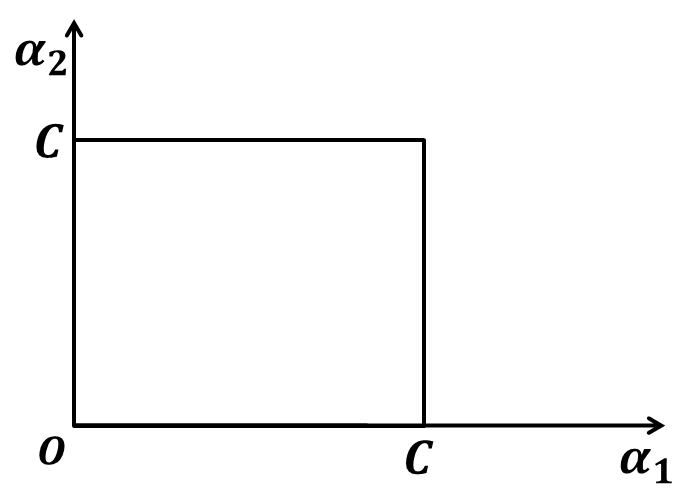
\includegraphics[height=4cm]{images/SMOBinary_quadratic_programming.jpg}
            \caption{SMO二元二次规划图1}
            \label{SMO二元二次规划图1}
            \end{figure}
        图(\ref{SMO二元二次规划图1})给出了变量$\alpha_1,\alpha_2$的取值范围,接着,我们约束$\alpha_1y_1+\alpha_2y_2 = \xi$,此约束需要分情况讨论:
        \par
        (1)当$y_1,y_2$同号时,有$\alpha_1+\alpha_2 = \xi$,那么我们就要讨论$\xi $和$c$的大小,当$\xi <c$时,$\alpha_1,\alpha_2$的直线就如图(\ref{SMO二元二次规划图2})(a)下直线所示;当$\xi > c$时,$\alpha_1,\alpha_2$的直线就如图(\ref{SMO二元二次规划图2})(a)上直线所示。由此我们有$\alpha_2$的取值
        \begin{align*}
        & L = \max(0,\xi-c)\\
        & H=\min(c,\xi)\\
        & L \leqslant \alpha_2^{new} \leqslant H
        \end{align*}
        \par
        (2)当$y_1,y_2$异号时,有$\alpha_1-\alpha_2 = \xi$,我们仍然要讨论$\xi $和$c$的大小,当$\xi <c$时,$\alpha_1,\alpha_2$的直线就如图(\ref{SMO二元二次规划图2})(b)上直线所示;当$\xi < c$时,$\alpha_1,\alpha_2$的直线就如图(\ref{SMO二元二次规划图2})(b)下直线所示。由此我们有$\alpha_2$的取值
        \begin{align*}
        & L = \max(0,\xi-c)\\
        & H=\min(c,\xi+c)\\
        & L \leqslant \alpha_2^{new} \leqslant H
        \end{align*}
			\begin{figure}[H]
			  \centering
			  \begin{varwidth}[t]{\textwidth}
			    \vspace{0pt}
			    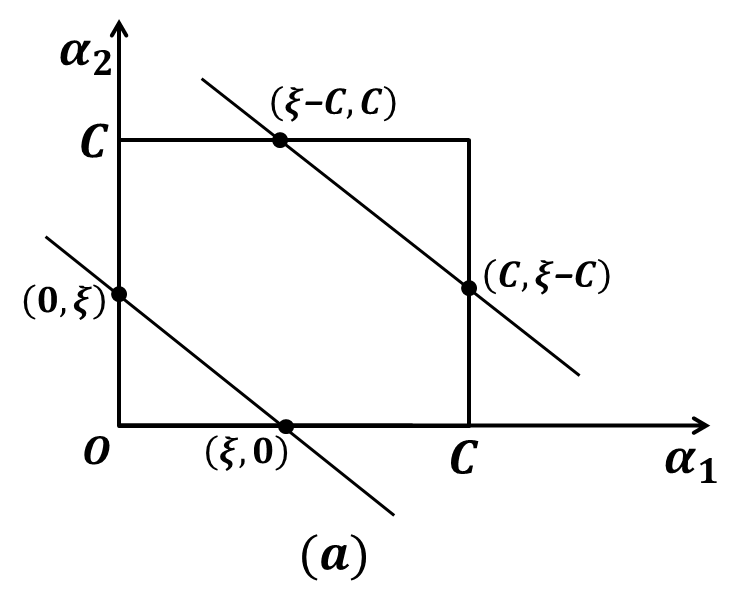
\includegraphics[height=4cm]{images/Binary_quadratic_programming1.jpg}
			  \end{varwidth}
			  \qquad
			  \begin{varwidth}[t]{\textwidth}
		    \vspace{0pt}
		    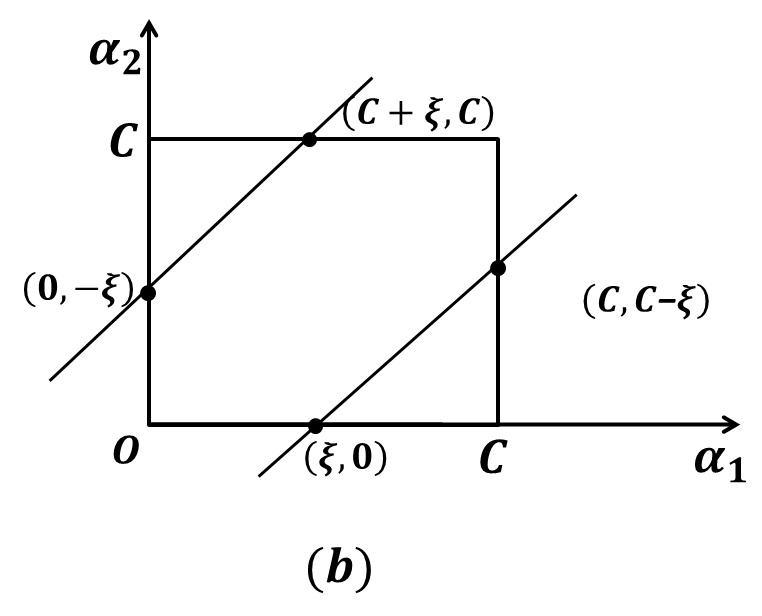
\includegraphics[height=4cm]{images/Binary_quadratic_programming2.jpg}
 		 \end{varwidth}
            \caption{SMO二元二次规划图2}
            \label{SMO二元二次规划图2}
            \end{figure}
        \par
        设$\alpha_1^{old},\alpha_2^{old}$为更新前的点,$\alpha_1^{new},\alpha_2^{new}$为更新后的点。由$\alpha_1y_1+\alpha_2y_2 = \xi$得到
        \begin{align*}
        \alpha_1 = (\xi-\alpha_2y_2)/y_1 = (\xi-\alpha_2y_2)y_1
        \end{align*}
        将目标$J$中的$\alpha_1$用上式替换,有
        \begin{align*}
        \min_{\alpha_2} \ W(\alpha_2) &= \frac{1}{2}k_{11}(\xi -\alpha_2y_2)^2 + \frac{1}{2}\alpha_2^2k_{22}+y_1y_2(\xi -\alpha_2y_2)y_1\alpha_2k_{12}\\
        &\quad + (\xi-\alpha_2y_2)y_1y_1v_1+\alpha_2y_2v_2 - (\xi-\alpha_2y_2)y_1 - \alpha_2 +\psi_{constant}\\
        & =\frac{1}{2}k_{11}(\xi-\alpha_2y_2)^2+\frac{1}{2}k_{22}\alpha_2^2 +y_2\alpha_2k_{12}(\xi-\alpha_2y_2)\\
        &\quad+(\xi-\alpha_2y_2)v_1+\alpha_2y_2v_2-(\xi-\alpha_2y_2)y_1-\alpha_2+\psi_{constant}
        \end{align*}
        因为要求$\min\limits_{\alpha_2}$,所以目标函数$W(\alpha_2)$对$\alpha_2$求导,令导数为零以求取极值,有
        \begin{align*}
        \frac{\partial W}{\partial \alpha_2} = k_{11}\alpha_2 +k_{22}\alpha_2 - 2k_{12}\alpha_2 - k_{11}\xi y_2 +k_{12}\xi y_2+y_1y_2-1-v_1y_2+v_2y_2 = 0
        \end{align*}
        由上式推得
        \begin{align*}
        (k_{11}+k_{22}-2k_{12})\alpha_2 = y_2(y_2-y_1+\xi k_{11}-\xi k_{12}+v_1-v_2)
        \end{align*}
        将$\xi = \alpha_1^{old}y_1+\alpha_2^{old}y_2$和$v_1,v_2$带入上式,有
        \begin{align*}
        (k_{11}+k_{22}-2k_{12})\alpha_2 &= y_2 \Big[y_2-y_1 +(\alpha_1^{old}y_1+\alpha_2^{old}y_2)(k_{11}-k_{12}) \\
        &\quad +\underline{\sum_{j=3}^n \alpha_jy_jk(x_1,x_j)} - \underline{\sum_{j=3}^n\alpha_jy_jk(x_2,x_j)} \Big]\\
        &= y_2 \Bigg[y_2-y_1 +(\alpha_1^{old}y_1+\alpha_2^{old}y_2)(k_{11}-k_{12}) \\
        &\quad + \left( \sum_{j=1}^n \alpha_jy_jk(x_1,x_j) - \alpha_1y_1k_{11} - \alpha_2 y_2k_{12} \right) \\
        &\quad - \left( \sum_{j=1}^n \alpha_jy_jk(x_2,x_j) - \alpha_1y_1k_{21} - \alpha_2 y_2k_{22}  \right) \Bigg]\\
        & = y_2[y_2-y_1+g(x_1)-g(x_2)+\alpha_2^{old}y_2(k_{11}+k_{22}-2k_{12})]
        \end{align*}
        其中:$g(x_1) = \sum\limits_{j=1}^n \alpha_jy_jk(x_1,x_j), g(x_2) = \sum\limits_{j=1}^n \alpha_jy_jk(x_2,x_j)$。
        \par
        令$E_i = \sum_{i=1}^n\alpha_iy_ik(x_i,x_j)+b-y_i$为估计值与真实值之差,$\eta = k_{11}+k_{12}-2k_{12}$。上式两边同除$\eta$,有
        \begin{align*}
        \alpha_2 = \alpha_2^{old}+\frac{y_2(E_1-E_2)}{\eta}
        \end{align*}
        由于$\alpha_2$有取值范围$L \leqslant \alpha_2 \leqslant H$,于是$\alpha_2$为
        \begin{align*}
        \alpha_2^{new,clipped} = \left\{
        \begin{aligned}
        & H\quad&  H \leqslant \alpha_2^{new}\\
        & \alpha_2^{new}\quad&  L < \alpha_2^{new} <H\\
        & L \quad&  \alpha_2^{new} \leqslant L
        \end{aligned}
        \right.
        \end{align*}
        与此同时,$\alpha_1^{new} = \alpha_1^{old}+\frac{y_1E_1}{k_{11}}$。令$s= y_1y_2$,最终的$\alpha_1$的更新公式为
        \begin{align*}
        \alpha_1^{new} = \alpha_1^{old}+s(\alpha_2-\alpha_2^{new,clipped})
        \end{align*}
        \par
        至此,我们已经给出其他参数的更新公式。但上述求解过程有一个问题,即$\eta$的取值,如果$\eta $为0,则不可以将其作为分母。Platt在其论文中讨论了$\eta$的特殊情况:如果核$K$不满足Mercer定理,那么目标函数可能变得非正,$\eta$可能取负。即使$K$是有效核,如果训练集中出现相同的$x$,那么$\eta$有可能为0。SMO算法在$\eta$非正时仍有效:我们可以推导出$\frac{\partial^2 W}{\partial \alpha_2^2}=\eta$,当$\eta<0$时,$W$没有极小值,最小值在边缘取得;当$\eta>0$时,$W$更为单调函数,最小值也在边缘处取得。而$\alpha_2$的边缘即为$L$和$H$,这样,将$\alpha_2 = L$和$\alpha_2 = H$带入$W$中即可求得$W$最小值,将$\alpha_2$修正到目标函数$W(L),W(H)$较小的端点上,$\alpha_2 = L/H$。具体计算公式为
        \begin{align*}
        & f_1 = y_1(E_1+b)-\alpha_1k(x_1,x_1)-s\alpha_2k(x_1,x_2)\\
        & f_2 = y_2(E_2+b)-s\alpha_1k(x_1,x_2)-\alpha_2k(x_2,x_2)\\
        & L_1 = \alpha_1+s(\alpha_2-L)\\
        & H_1 = \alpha_1 + s(\alpha_2-H)\\
        & W_L = L_1f_1+L f_2+\frac{1}{2}L_1^2k(x_1,x_1)+\frac{1}{2}L^2k(x_2,x_2)+sLL_1k(x_1,x_2)\\
        & W_H = H_1f_1+Hf_2+\frac{1}{2}H_1^2k(x_1,x_1)+\frac{1}{2}H^2k(x_2,x_2)+sHH_1k(x_1,x_2)
        \end{align*}
        \par
        下面,我们来更新阈值$b$和差值$E_i$。在每次完成$\alpha_1,\alpha_2$的更新后,都要重新计算$b$和$E$。
        \par
        (1)当$0<\alpha_1^{new}<c$时,有
        \begin{align*}
        \sum_{i=1}^n \alpha_iy_ik_{i1}+b = y
        \end{align*}
        由此可得
        \begin{align*}
        b_1^{new} = y_1-\sum_{i=3}^n\alpha_iy_ik_{i1}-\alpha_1^{new}y_1k_{11}-\alpha_2^{new}y_2k_{21}
        \end{align*}
        我们知道$E_i = \sum_{j=1}^n\alpha_j y_jk(x_j,x_i)+b-y_i  $,由此,我们得到
        \begin{align*}
        E_1 = \sum_{i=3}^n\alpha_i y_ik_{k1}+\alpha_1^{old}y_1k_{11}+\alpha_2^{old}y_2k_{21}+b^{old}-y_1
        \end{align*}
        将$E_1$带入到上面$b_1$的更新公式,有
        \begin{align*}
        b_1^{new} &= -E_1 + \alpha_1^{old}y_1k_{11}+\alpha_2^{old}y_2k_{21}+b^{old}-\alpha_1^{new}y_1k_{11}-\alpha_2^{new}y_2k_{21}\\
        &=-E_1-y_1k_{11}(\alpha_1^{new}-\alpha_1^{old})+y_2k_{21}(\alpha_2^{new}-\alpha_2^{old})+b^{old}
        \end{align*}
        同理,我们有$b_2$的更新公式
        \begin{align*}
        b_1^{new} =-E_2-y_1k_{11}(\alpha_1^{new}-\alpha_1^{old})+y_2k_{22}(\alpha_2^{new}-\alpha_2^{old})+b^{old}
        \end{align*}
        \par
        (2)如果$\alpha_1^{new},\alpha_2^{new}$同时满足$0<\alpha_i^{new}<c$,即两个Langrange乘子都在界内,则$b^{new}_1=b_2^{new}$。
        \par
        (3)如果$\alpha_1^{new},\alpha_2^{new}$是0或者$c$,即两个Langrange乘子都在边界上,$b_1,b_2$以及它们之间的都可以作为符合KKT条件的阈值,Platt采用$b = \frac{b_1+b_2}{2}$来处理。
        \par
        $E_i$值的更新要用到$b^{new}$,以及所有支持向量对应的$\alpha_j$
        \begin{align*}
        E_1^{new} = \sum_{s} y_j\alpha_j k(x_i,x_j)+b^{new} - y_i
        \end{align*}
        其中:$s$为支持向量$x_j$的集合。
        \subsubsection{工作集$B$的确定}
            \par
            下面,我们来介绍工作集$B$的确定。Platt的SMO算法每次修改$E_i$都涉及到$b$,Keerthi提出一种不考虑$b$的KKT条件判别法:设$F_i = \sum_{j=1}^n\alpha_jy_j k(x_i,x_j)-y_i$有
            \begin{align*}
            F_i = E_i-b
            \end{align*}
            于是KKT条件变为
            \begin{align*}
            \alpha_i = 0 \Rightarrow y_i (F_i+b) \geqslant 0\\
            0<\alpha_i <c \Rightarrow y_i (F_i+b) = 0\\
            \alpha_i = 0 \Rightarrow y_i (F_i+b) \leqslant 0
            \end{align*}
            \par
            引入符号
            \begin{align*}
            I_0 = \{i:0<\alpha_i<c\} \quad F_i = -b\\
            I_1 = \{i:y_i \pm 1\ \& \ \alpha_i=0\} \quad F_i \geqslant -b\\
            I_2 = \{i:y_i = -1\ \&\ \alpha_i=c\} \quad F_i \geqslant -b\\
            I_3 = \{i:y_i = +1\ \&\ \alpha_i=c\} \quad F_i \leqslant -b\\
            I_4 = \{i:y_i=-1\ \&\ \alpha_i>0\} \quad F_i \leqslant -b\\
            \end{align*}
            则KKT条件可表示为
            \begin{align*}
            i\in I_0 \cup I_1\cup I_2 \Rightarrow F_i \geqslant -b\\
            i\in I_0 \cup I_3\cup I_4 \Rightarrow F_i \leqslant -b
            \end{align*}
            当KKT条件满足时,$\forall i\in I_0 \cup I_1\cup I_2, \forall j\in I_0\cup I_3\cup I_4$,有$F_i \geqslant -b \geqslant F_j$。设
            \begin{align*}
            b_{low} = \max\{-F_i:i\in I_0\cup I_1\cup I_2\}\\
            b_{up} = \min\{-F_j:j\in I_0\cup I_3\cup I_4\}
            \end{align*}
            当KKT条件满足时,有$b_{up} \geqslant b_{low}$。这样就可以通过直接计算$b_{up} \geqslant b_{low}$,而不是每次先更新$b$值再来判断所得的解是否满足KKT。Keerthi工作集$B$的选取为
            \begin{align*}
            i &= \max \left( \{-y_tF_t|y_t=1,\alpha_t <c\}\cup \{y_tF_t|y_t=-1,\alpha_t>0\} \right) \\
            &=\max \left( -F_t\{y_t=1,\alpha_t <c\}\cup \{y_t=-1,\alpha_t>0\} \right) \\
            j &= \max \left( \{y_tF_t|y_t=-1,\alpha_t <c\}\cup \{-y_tF_t|y_t=1,\alpha_t>0\} \right) \\
            &=\max \left( -F_t\{y_t=-1,\alpha_t <c\}\cup \{y_t=1,\alpha_t>0\} \right)
            \end{align*}
            算法结束后,有$b = \frac{b_{up}+b_{low}}{2}$。
            \par
            上面介绍了Keerthi工作集$B$的选取方法,下面简单介绍Fan的方法。For all $t,s$ define
            \begin{align*}
            &a_{ts} = k_{tt} +k_{ss}-2k_{ts}\\
            &b_{ts} = -y_t\nabla f(\alpha^k)_t+y_s\nabla f(\alpha^k)_s>0\\
            &\bar{a}_{ts} = \left\{
            \begin{aligned}
            a_{ts}\quad a_{ts}>0\\
            \tau \quad otherwise
            \end{aligned}
            \right.
            \end{align*}
            select
            \begin{align*}
            & i\in \max_t \left\{ -y_t\nabla f(\alpha^k)_t|t\in I_{up}(\alpha^k) \right\}\\
            & j\in \min \left\{\frac{b_{it}^2}{\bar{a}_{it}}|i\in I_{low}(\alpha^k),-y_t\nabla f(\alpha^k)<-y_t\nabla f(\alpha^k)_i  \right\}
            \end{align*}
            where
            \begin{align*}
            I_{up}(\alpha) = \{t|\alpha_t <c,y_t=1\ \mathrm{or}\ \alpha_t>0,y_t=-1\}\\
            I_{low}(\alpha) = \{t|\alpha_t <c,y_t=-1\ \mathrm{or}\ \alpha_t>0,y_t=1\}
            \end{align*}


\section{支持向量回归}
    \par
    前一部分我们建立了二分类支持向量机,二分类标签为$y=\{-1,1\}$。接下来我们讨论$y$是连续型数值的情况,即回归问题。用于处理回归问题的支持向量机被称为支持向量回归SVR。(此处应该注意,我们仍然强调支持向量的概念,如果不存在支持向量,那么这种方法也就称不上支持向量机了)。为了研究简便,我们考虑二元回归$y=f(x)$,$x,y\in R$的情况。我们来看一些可能的回归问题,如图(\ref{二元回归问题示意图})所示
			\begin{figure}[H]
			  \centering
			  \begin{varwidth}[t]{\textwidth}
			    \vspace{0pt}
			    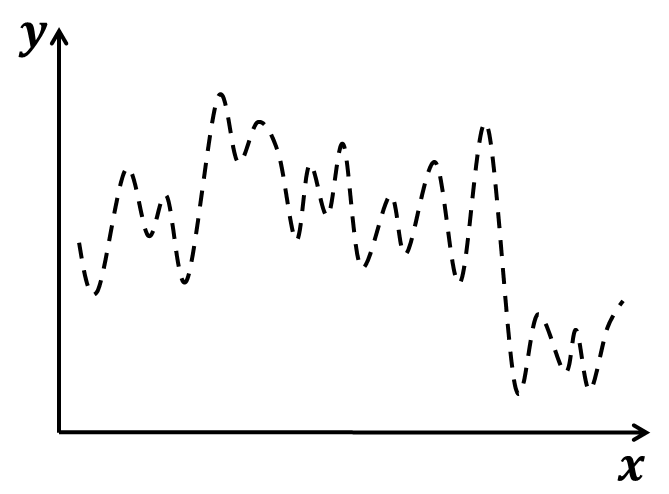
\includegraphics[height=4cm]{images/Binary_regression1.jpg}
			  \end{varwidth}
			  \qquad
			  \begin{varwidth}[t]{\textwidth}
			    \vspace{0pt}
			    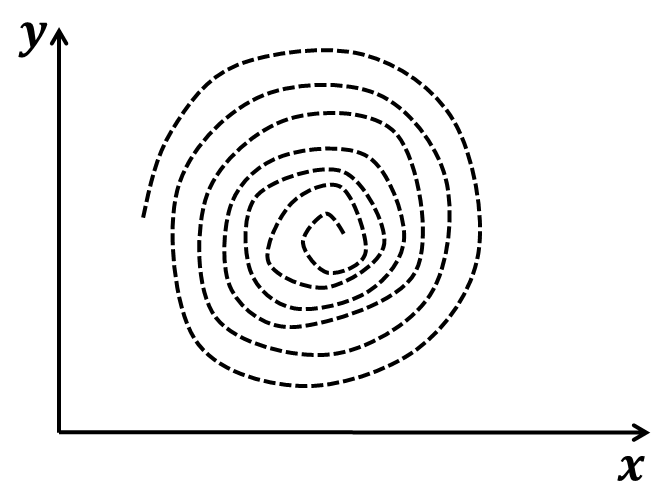
\includegraphics[height=4cm]{images/Binary_regression2.jpg}
 			 \end{varwidth}
            \caption{二元回归问题示意图}
            \label{二元回归问题示意图}
            \end{figure}
    \par
    和前面的研究思路一样,我们仍从线性回归模型出发,最后利用核技术将其投影成非线性问题。支持向量回归SVR问题如图(\ref{支持向量回归示意图})所示
		\begin{figure}[H]
		\centering
		\begin{varwidth}[t]{\textwidth}
		\vspace{0pt}
		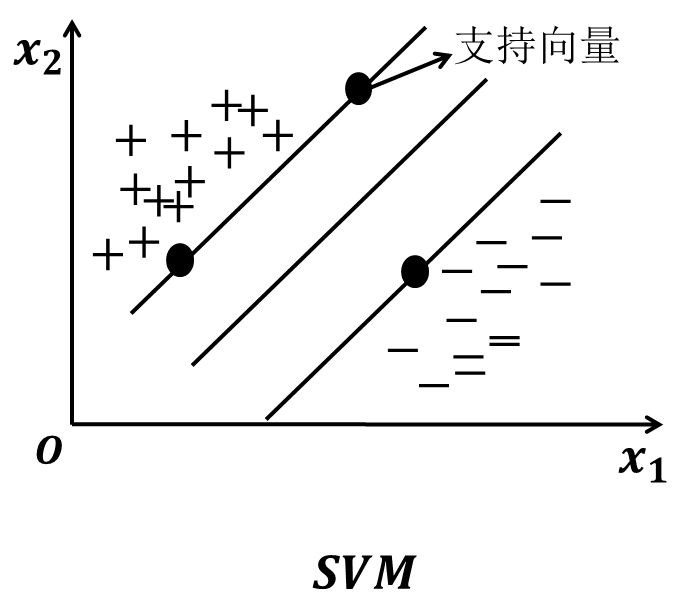
\includegraphics[height=4cm]{images/Support_vector_regression1.jpg}
		\end{varwidth}
		\qquad
		\begin{varwidth}[t]{\textwidth}
		\vspace{0pt}
		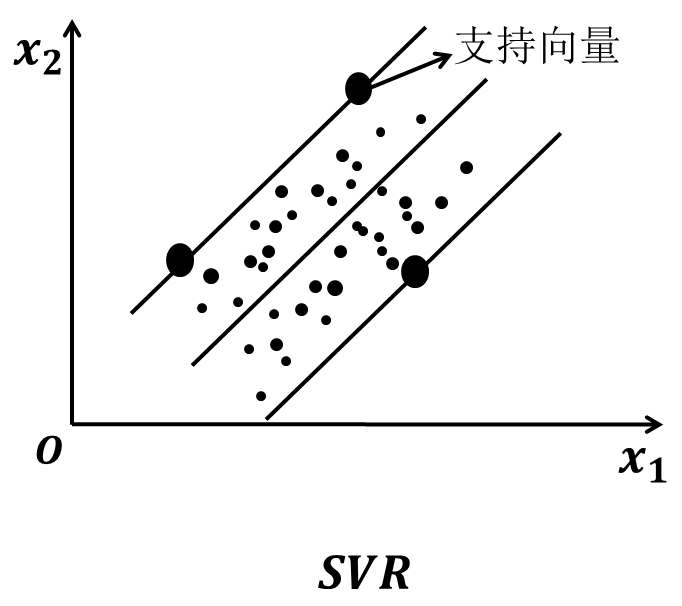
\includegraphics[height=4cm]{images/Support_vector_regression2.jpg}
		\end{varwidth}
            \caption{支持向量回归示意图}
            \label{支持向量回归示意图}
            \end{figure}
    回忆一下,在前面的2分类问题中,我们的目标是:求$w,b$,使得样本点到分割线/直线的最小距离最大。下面,我们来考虑回归问题的目标:
    \begin{enumerate}
    \item 求$w,b$,使得样本点到直线$f(x)$的总距离最小(距离可以是平方距离等);
    \item 求$w,b$,使得样本点到直线$f(x)$的最大距离最小(所有样本点落在区域内,且区域最小);
    \item 求$w,b$,使得样本点到直线$f(x)$的最小距离最大。
    \end{enumerate}
    \par
    上面第一个目标/方案是不错的,而且非常好,很像最小二乘回归(样本点到直线的总离差平方最小)。当然也可以使用最小一乘回归和最大离差回归,因为其不具备支持向量,所以我们暂时不做研究。下面,我们来描述一下第二个目标/方案:最大距离最小化,如图(\ref{最大距离最小化示意图})所示。为了方便,我们将$y$记为$x_2$
            \begin{figure}[H]
            \centering
            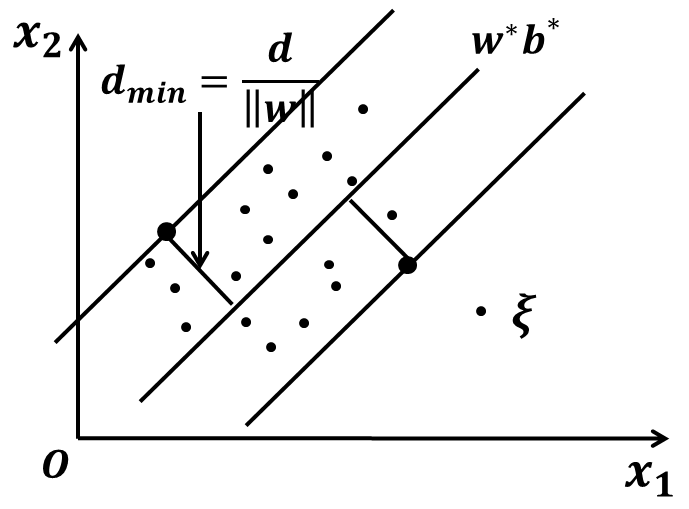
\includegraphics[height=4cm]{images/maxdistance_min.jpg}
            \caption{最大距离最小化示意图}
            \label{最大距离最小化示意图}
            \end{figure}
    首先,点到线的距离为
    \begin{align*}
    \frac{|w^\mathrm{T}x_i+b|}{||w||} = r_i
    \end{align*}
    最大距离最小化的目标为
    \begin{align*}
    \min_{w,b}\ \max_{i}\ \left\{ r_i = \frac{|w^\mathrm{T}x_i+b|}{||w||}\right\}
    \end{align*}
    记最大距离为$\frac{d}{||w||}$,重写上述目标有
    \begin{align*}
    & \min_{w,b} \ \frac{d}{||w||}\\
    & s.t.\left\{
    \begin{aligned}
    |w^\mathrm{T}x_i+b| \leqslant d\\
    i=1,2,\dots,n
    \end{aligned}
    \right.
    \end{align*}
    \par
    由于距离是相对的,不妨设最大距离的$d=1$,而其样本点的距离$<1$,于是有
    \begin{align}
    \label{支持向量回归最大最小模型目标1}
    & \min_{w,b} \ \frac{1}{||w||}\\
    & s.t.\left\{
    \begin{aligned}
    |w^\mathrm{T}x_i +b| \leqslant 1\\
    i=1,2,\dots,n
    \end{aligned}
    \right.\notag
    \end{align}
    也即$\max\limits_{w,b}\frac{1}{2}||w||^2$,即$\min\limits_{w,b}-\frac{1}{2}||w||^2$。设置容错量$\xi$,使得部分样本可以在距离外,即$|w^\mathrm{T}x_i+b| \leqslant 1+\xi_i,\xi_i \geqslant 0$。
    \par
    $\xi$的设置带来了损失,我们计算$w,b$时,$\xi$(“带”外的点)无效。为此我们使损失最小,有
    \begin{align}
    \label{支持向量回归最大最小模型目标2}
    \min_{w,b} \ \sum_{i=1}^n \xi_i
    \end{align}
    将上述目标(\ref{支持向量回归最大最小模型目标1})和目标(\ref{支持向量回归最大最小模型目标2})合并,并设置目标权重为$c$,有
    \begin{align*}
    & \min_{w,b,\xi} \ -\frac{1}{2}w^\mathrm{T}w +c \sum_{i=1}^n \xi_i\\
    & s.t.\left\{
    \begin{aligned}
    & |w^\mathrm{T}x_i+b| \leqslant 1+\xi_i\\
    & \xi \geqslant 0\\
    & i=1,2,\dots,n
    \end{aligned}
    \right.
    \end{align*}
    将上述模型中的不等式约束展开,有
    \begin{align*}
    & \min_{w,b,\xi,\xi^*} \ -\frac{1}{2}w^\mathrm{T}w +c \sum_{i=1}^n( \xi_i+\xi_i^*)\\
    & s.t.\left\{
    \begin{aligned}
    & w^\mathrm{T}x_i+b \leqslant 1+\xi_i\\
    & w^\mathrm{T}x_i+b \geqslant -1-\xi_i^*\\
    & \xi_i \geqslant 0\\
    & \xi_i^* \geqslant 0\\
    & i=1,2,\dots,n
    \end{aligned}
    \right.
    \end{align*}
    \par
    至此,最大距离最小模型已经建成。我们来看一下这个模型是否可求,当$\xi_i,\xi_i^*$增大时,相当于边界减小,$w,b$也会增大,$-w$会减小,即$\xi \uparrow,-w\downarrow$,所以有最优$w,b$是二者取中。不过困难的是,上述问题并非凸二次规划($\min x^\mathrm{T}Hx+cx$,$H$为半正定时,为凸规划),因为这里的$H$为$-I$(是负定的),所以我们不能用Langrange对偶方法对问题进行求解。
    \par
    下面,我们来考虑目标/方案3:使样本点到直线$f(x)$的最小距离最大。如图(\ref{最小距离最大化示意图})所示
            \begin{figure}[H]
            \centering
            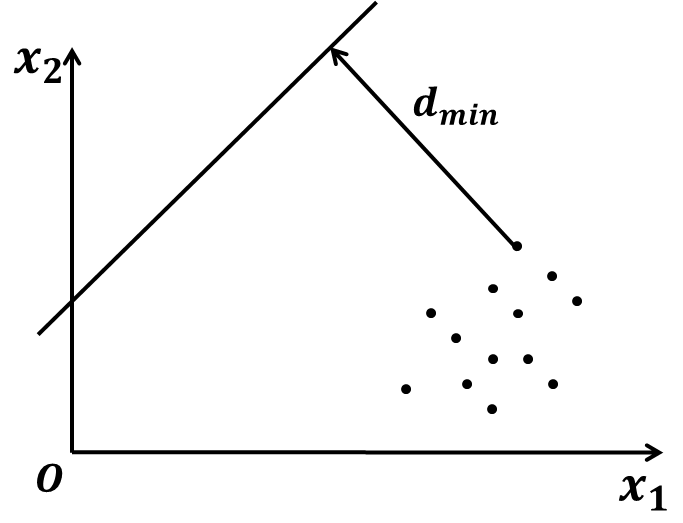
\includegraphics[height=4cm]{images/mindistance_max.jpg}
            \caption{最小距离最大化示意图}
            \label{最小距离最大化示意图}
            \end{figure}
    如果直接求取最小距离最大化的话,会出现如上图(\ref{最小距离最大化示意图})的情况:我们会让直线$f(x)$尽可能的向远处走,甚至是无穷大。这样是不好的,我们希望将直线约束在一定的范围内(数据点到直线的距离是有限的),比如$|y_i - w^\mathrm{T}x_i-b| < \epsilon$,换句话说,我们是将数据点放在一个“带”内,这个“带”就是两个直线$|y_i - w^\mathrm{T}x_i-b| < \epsilon$构成的。并且,这种最小距离最大并不好,毕竟我们没有必要要求最小距离最大(二分类支持向量机的目标)。
    \par
    上面三个目标/方案都不是很好,下面,我们在二分类支持向量机的模型上进行思考
    \begin{align*}
    & \min_{w,b,\xi} \ \frac{1}{2}||w||^2+c\sum_{i=1}^n\xi_i \\
    & s.t.\left\{
    \begin{aligned}
    & y_i(w^\mathrm{T}\varphi(x_i)+b) \geqslant 1-\xi_i\\
    & \xi_i \geqslant 0, i=1,2,\dots,n
    \end{aligned}
    \right.
    \end{align*}
    其实,上面这种模型可以有另一种解释:我们将$\xi_i$视为观测值$y_i$和理论值$w^\mathrm{T}\varphi(x_i)+b$的误差,则目标中的$\sum_{i=1}^n\xi_i$部分是表示误差和最小;和回归模型相比,$||w||^2$可视为正则项,$||w||$会使得拟合函数更加平滑。这里的损失函数就是Huber损失,只有当$y_i$和$w^\mathrm{T}\varphi(x_i)+b$超过一定界限时($y_i(w^\mathrm{T}\varphi(x_i)+b) \geqslant 1-\xi_i$),才计算误差,否则误差为0。
    \par
    对于回归问题,我们仍将$\xi_i$视为$y_i$和$w^\mathrm{T}\varphi(x_i)+b$的误差,我们要求误差总和最小。仍采用Huber损失,Huber损失的阈值设为$\varepsilon$,有
    \begin{align*}
    y_i - f(x_i) \leqslant \varepsilon + \xi_i  \\
    f(x_i) - y_i \leqslant \varepsilon + \xi_i^*
    \end{align*}
    这里的$\xi_i,\xi_i^*$为误差。建立支持向量回归模型
    \begin{align*}
    & \min_{w,b,\xi,\xi^*} \ J(w,b,\xi,\xi^*) = c\sum_{i=1}^n (\xi_i+\xi_i^*) \\
    & s.t.\left\{
    \begin{aligned}
    & y_i - f(x_i) \leqslant \varepsilon + \xi_i  \\
    & f(x_i) - y_i \leqslant \varepsilon + \xi_i^* \\
    & \xi_i,\xi_i^*\geqslant 0\\
    & i=1,2,\dots,n
    \end{aligned}
    \right.
    \end{align*}
    我们在上面的模型中添加正则项$||w||$,有
    \begin{align*}
    & \min_{w,b,\xi,\xi^*} \ J(w,b,\xi,\xi^*) = c\sum_{i=1}^n (\xi_i+\xi_i^*) + \frac{1}{2}||w||^2\\
    & s.t.\left\{
    \begin{aligned}
    & y_i - f(x_i) \leqslant \varepsilon + \xi_i  \\
    & f(x_i) - y_i \leqslant \varepsilon + \xi_i^* \\
    & \xi_i,\xi_i^*\geqslant 0\\
    & i=1,2,\dots,n
    \end{aligned}
    \right.
    \end{align*}
    \par
    上述问题是一个凸二次规划问题,引入Langrange函数
    \begin{align*}
    L &= \frac{1}{2}||w|| + c\sum_{i=1}^n(\xi_i+\xi_i^*) -\sum_{i=1}^n \alpha_i [\xi_i+\varepsilon -y_i +f(x_i)] \\
    &\quad - \sum_{i=1}^n\alpha_i^* [\xi_i^* +\varepsilon-y_i +f(x_i)] - \sum_{i=1}^n(\xi_ir_i+\xi_i^*r_i^*)
    \end{align*}
    其中:$\alpha_i,\alpha_i^*,r_i,r_i^*$为Langrange算子,$\alpha_i^*,r_i^* \geqslant 0$。求$L$对$w,b,\xi,\xi^*$最小,对$\alpha_i,\alpha_i^*,r_i,r_i^*$最大,推导$L$有
    \begin{align*}
    & \max_{\alpha,\alpha^*} \ W(\alpha,\alpha^*) = \frac{1}{2}\sum_{i=1}^n\sum_{j=1}^n(\alpha_i - \alpha_i^*)(\alpha_j - \alpha_j^*)k(x_i,x_j)+\sum_{i=1}^n(\alpha_i-\alpha_i^*)y_i-\sum_{i=1}^n (\alpha_i+\alpha_i^*)\varepsilon\\
    & s.t.\left\{
    \begin{aligned}
    & \sum_{i=1}^n (\alpha_i-\alpha_i^*) = 0\\
    & 0 \leqslant \alpha_i,\alpha_i^* \leqslant c
    \end{aligned}
    \right.
    \end{align*}
    将上式写为二次规划问题为
    \begin{align*}
    & \min_{\alpha,\alpha^*}\ \frac{1}{2}(\alpha-\alpha^*)^\mathrm{T}Q(\alpha-\alpha^*) - \varepsilon \sum_{i=1}^n (\alpha_i+\alpha_i^*) + \sum_{i=1}^n (\alpha_i- \alpha_i^*)y_i\\
    & s.t.\left\{
    \begin{aligned}
    & \sum_{i=1}^n (\alpha_i-\alpha_i^*) = 0\\
    & 0 \leqslant \alpha_i,\alpha_i^* \leqslant c
    \end{aligned}
    \right.
    \end{align*}
    由KKT条件,在鞍点处
    \begin{align*}
    & \alpha_i [\varepsilon +\xi_i-y_i +f(x_i)] = 0\\
    & \alpha_i^* [\varepsilon +\xi_i^*-y_i +f(x_i)] = 0\\
    & \xi_i r_i = 0\\
    & \xi_i^* r_i^* = 0
    \end{align*}
    由上式可以推得$\alpha_i\alpha_i^* = 0$,所以$\alpha_i,\alpha_i^*$不同时为0。同时,我们得到
    \begin{align*}
    & (c-\alpha_i)\xi =0\\
    & (c-\alpha_i^*)\xi^* =0
    \end{align*}
    \ding{172}当$\alpha_i = c$或者$\alpha_i^* = c$时,$|f(x_i) - y_i|$可能大于$\varepsilon$,与其对应的$x_i$称为边界支持向量(Boundary Support Vector);\ding{173}当$\alpha_i^*\in (0,c)$时,$|f(x_i) - y_i| = \varepsilon$,即$\xi_i\xi_i^* = 0$与其对应的向量$x_i$称为标准支持向量(Normol Support Vector);\ding{174}当$\alpha_i^*,\alpha_i=0$时,$x_i$为非支持向量,它们对$w$没有影响,因此$\varepsilon$越大,支持向量越多。BSV、NSV如图(\ref{边界及标准支持向量示意图})所示
            \begin{figure}[H]
            \centering
            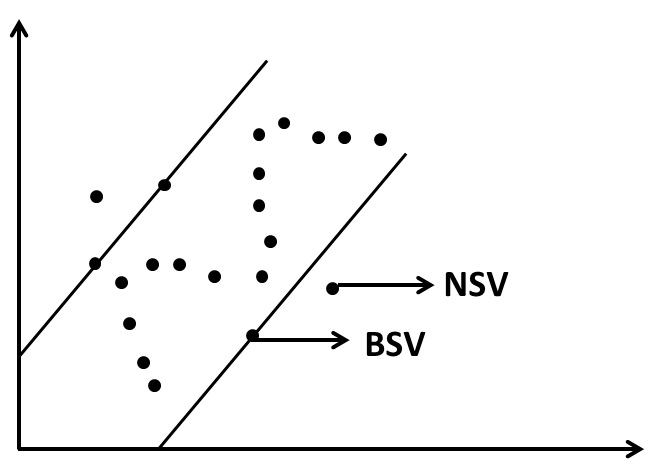
\includegraphics[height=4cm]{images/Boundary_and_Standard_Support_Vector.jpg}
            \caption{边界及标准支持向量示意图}
            \label{边界及标准支持向量示意图}
            \end{figure}
    \par
    对于NSV,$0<\alpha_i<c(\alpha_i^* = 0)$,此时$\xi_i=0$。由KKT可以求出$b$
    \begin{align*}
    b & = y_i - \sum_{j=1}^n(\alpha_i-\alpha_j^*)x_jx_i - \varepsilon\\
    & =y_i - \sum_{x_j\in SV}(\alpha_j - \alpha_j^*) x_jx_i -\varepsilon
    \end{align*}
    而对于$0<\alpha_i^*<c(\alpha_i=0)$的NSV,有
    \begin{align*}
    b = y_i - \sum_{x_j\in SV}(\alpha_j - \alpha_j^*) x_jx_i -\varepsilon
    \end{align*}
    一般对所有标准支持向量分别计算$b$,然后求平均值
    \begin{align*}
    b=\frac{1}{N_{NSV}} \left\{ \sum_{0<\alpha_i<c} \Big[ y_i - \sum_{x_j\in SV}(\alpha_j - \alpha_j^*)k(x_j,x_i)-\varepsilon\Big] + \sum_{0<\alpha_i^*<c} \Big[ y_i - \sum_{x_j\in SV}(\alpha_j - \alpha_j^*)k(x_j,x_i)-\varepsilon\Big] \right\}
    \end{align*}
    \par
    关于LSSVM解的稀疏性:大部分Langrange乘子$\alpha_i,\alpha_i^*$都等于0,样本数据只有少量支持向量。这个性质是由$\varepsilon$不敏感性引起的。通过增加或减少$\varepsilon$值,可以控制支持向量的个数,也即可控制SVR解的稀疏性。从解的稀疏性可以看出,其实很多样本是冗余的,在拟合过程中只有那些支持向量起作用,由此可以引导出下面的最小二乘支持向量机。
    \par
    LIBSVM工具包还提供了Scholkopf提出的$\nu$-SVR的求解。Scholkoph引入新的参数$\nu$来反应超出$\varepsilon$带之外样本数据点和支持向量数。$\nu$-SVR模型如下
    \begin{align*}
    & \min_{w,b,\xi,\xi^*,\varepsilon}\ \frac{1}{2}||w||+c(\nu\varepsilon+\frac{1}{n}\sum_{i=1}^n(\xi_i,x_i^*))\\
    & s.t.\left\{
    \begin{aligned}
    & y_i - w^\mathrm{T}\varphi(x_i)-b \leqslant \varepsilon +\xi_i\\
    & w^\mathrm{T}\varphi(x_i)+ b-y_i  \leqslant \varepsilon +\xi_i^*\\
    & \xi_i,\xi_i^* \geqslant 0\\
    & i=1,2,\dots,n
    \end{aligned}
    \right.
    \end{align*}
    其对偶模型为
    \begin{align*}
    & \min_{\alpha,\alpha^*}\ \frac{1}{2} (\alpha-\alpha^*)^\mathrm{T}Q(\alpha-\alpha^*) + y^\mathrm{T}(\alpha-\alpha^*)\\
    & s.t.\left\{
    \begin{aligned}
    & e^\mathrm{T}(\alpha - \alpha^*) = 0\\
    & e^\mathrm{T}(\alpha + \alpha^*) \leqslant c\nu\\
    & 0 \leqslant \alpha_i,\alpha_i^* \leqslant c/n
    \end{aligned}
    \right.
    \end{align*}
    为简化,不等式 $e^\mathrm{T}(\alpha+\alpha^*) \leqslant c\nu$ 用等式替代。在LIBSVM中,我们考虑 $c \leftarrow c/l$,所以有如下等价问题:
    \begin{align*}
    & \min_{\alpha,\alpha^*}\ \frac{1}{2} (\alpha-\alpha^*)^\mathrm{T}Q(\alpha-\alpha^*) + y^\mathrm{T}(\alpha-\alpha^*)\\
    & s.t.\left\{
    \begin{aligned}
    & e^\mathrm{T}(\alpha - \alpha^*) = 0\\
    & e^\mathrm{T}(\alpha + \alpha^*) \leqslant cn\nu\\
    & 0 \leqslant \alpha_i,\alpha_i^* \leqslant c
    \end{aligned}
    \right.
    \end{align*}

\section{多分类支持向量机}
    \par
    支持向量机虽然可以直接用于多分类问题,但是并不是很方便。对于多分类问题,我们可以将其转化为多个二分类问题进行求解,基于这一思想,会产生许多方法,这里我们不做详细介绍。

\section{最小二乘支持向量机}
    \par
    无论是SVR还是SVM,Vaonik等提出的原始支持向量机都需要借一个带不等式约束的二次规划问题。1999年,基于等式约束和最小二乘损失函数,Suykens和Vandewalle提出了求解二分类问题的最小二乘支持向量机LSSVM。LSSVM与标准SVM相比,减少了一个调整参数,减少了$n$个优化变量,从而简化计算,然而LSSVM没有保留解的稀疏性。改进的LSSVM有递推LSSVM、加权LSSVM、多分辨LSSVM、正则化LSSVM。
    \subsection{分类问题}
        \par
        对二分类问题$\{x^k,y^k\}_{k=1}^n,x^k\in R^m,y^k\in \{-1,1\}$,1999年Suykens给出的最小二乘支持向量模型如下
        \begin{align*}
        & \min_{w,b,\xi}\ J(w,b,\xi) = \frac{1}{2}w^\mathrm{T}w+\frac{\gamma}{2}\sum_{i=1}^n \xi_i^2\\
        & s.t.\quad y_i(w^\mathrm{T}\varphi(x_i)+b) = 1-\xi_i\\
        &\qquad  i=1,2,\dots,n
        \end{align*}
        其中:$\xi_i$是容错变量,$\gamma$为目标权重,$\sum\limits_{i=1}^n\xi_i^k$为正则化项。
        \par
        为求解上述优化问题,引入Langrange乘子$\alpha$,上述优化问题的Langrange函数为
        \begin{align*}
        L(w,b,\xi,\alpha) = J(w,b,\xi) - \sum_{i=1}^n \alpha_i [y_i(w^\mathrm{T}\varphi(x_i)+b)-1+\xi_i]
        \end{align*}
        称$\alpha_i \neq 0$的样本点为支持向量。根据KKT条件可得到
        \begin{align*}
        & \frac{\partial L}{\partial w} = 0 \quad \Rightarrow\quad w = \sum_{i=1}^n\alpha_iy_i\varphi(x_i)\\
        & \frac{\partial L}{\partial b}=0 \quad \Rightarrow \quad\sum_{i=1}^n \alpha_iy_i = 0\\
        & \frac{\partial L}{\partial \xi_i} = 0\quad \Rightarrow \quad\alpha_i = \gamma \xi_i\quad i=1,2,\dots,n\\
        & \frac{\partial L}{\partial \alpha_i} = 0\quad \Rightarrow \quad y_i(w^\mathrm{T}\varphi(x_i)+b)-1+\xi_i = 0\quad i=1,2,\dots,n
        \end{align*}
        消元去掉$\xi_i,w$,可以得到下面的线性方程组
        \begin{align*}
        \begin{bmatrix}
        I & 0 & 0 & -Z^\mathrm{T}\\
        0 & 0 & 0 & -y^\mathrm{T}\\
        0 & 0 & cI&  -I\\
        Z & y & I & 0
        \end{bmatrix}
        \begin{bmatrix}
        w\\
        b\\
        \xi\\
        \alpha
        \end{bmatrix}
        =\begin{bmatrix}
        0\\
        0\\
        0\\
        1_{n}
        \end{bmatrix}
        \end{align*}
        最后写成矩阵的形式有
        \begin{align*}
        \begin{pmatrix}
        0 & y^\mathrm{T}\\
        y& ZZ^\mathrm{T}+\gamma^{-1}I
        \end{pmatrix}
        \begin{pmatrix}
        b\\
        \alpha
        \end{pmatrix}
        =\begin{pmatrix}
        0\\
        1_{n}
        \end{pmatrix}
        \end{align*}
        其中:$Z = (\varphi(x_1)y_1,\dots,\varphi(x_n)y_n )^\mathrm{T}$,$y = (y_1,\dots,y_n)^\mathrm{T}$,$1_n=(1,\dots,1)^\mathrm{T}$,$\alpha = (\alpha_1,\dots,\alpha_n)^\mathrm{T}$。非线性函数分类$ZZ^\mathrm{T}$内积运算可用满足Mercer条件的核函数$k(x_i,x_j)$替代,令$\Omega = ZZ^\mathrm{T}$,则
        \begin{align*}
        \Omega_{ij} = y_iy_j\varphi(x_i)^\mathrm{T}\varphi(x_j)
        \end{align*}
        则上述方程可以表述为
        \begin{align*}
        \begin{pmatrix}
        0 & y^\mathrm{T}\\
        y & \Omega+\gamma^{-1}I
        \end{pmatrix}
        \begin{pmatrix}
        b\\
        \alpha
        \end{pmatrix}
        =\begin{pmatrix}
        0\\
        1_{n}
        \end{pmatrix}
        \end{align*}
        解上述方程得到$\alpha,b$后,对于新的输入向量/样本$x$,其分离可以根据下式进行判断
        \begin{align*}
        y(x) = \mathrm{sgn} \left[ \sum_{i=1}^n\alpha_iy_i k(x,x_i) +b \right]
        \end{align*}
    \subsection{回归问题}
        \par
        对于回归问题$\{x_i,y_i\}_{i=1}^n,x_i\in R^m,y_i\in R$,在Saunders, Gammerman和Vovk所提出的岭回归公式中,令$a = \frac{1}{\gamma}$,则最小二乘支持向量机的优化问题为
        \begin{align*}
        & \min_{w,b,\xi} \ J(w,b,\xi) = \frac{1}{2}w^\mathrm{T}w+\frac{\gamma}{2}\sum_{i=1}^n\xi_i^2\\
        & s.t. \quad y_i = w^\mathrm{T}\varphi(x_k)+b+\xi_i \quad i=1,2,\dots,n
        \end{align*}
        上面优化问题的Langrange函数为
        \begin{align*}
        L(w,b,\xi,\alpha) = J(w,b,\xi) - \sum_{i=1}^n \alpha_i (w^\mathrm{T}\varphi(x_i)+b+\xi_i-y_i)
        \end{align*}
        相应的KKT条件为
        \begin{align*}
        & \frac{\partial L}{\partial w} = 0 \quad \Rightarrow\quad w = \sum_{i=1}^n\alpha_i\varphi(x_i)\\
        & \frac{\partial L}{\partial b}=0 \quad \Rightarrow \quad\sum_{i=1}^n \alpha_i = 0\\
        & \frac{\partial L}{\partial \xi_i} = 0\quad \Rightarrow \quad\alpha_i = \gamma \xi_i\quad i=1,2,\dots,n\\
        & \frac{\partial L}{\partial \alpha_i} = 0\quad \Rightarrow \quad w^\mathrm{T}\varphi(x_i)+b+\xi_i - y_i = 0\quad i=1,2,\dots,n
        \end{align*}
        可以将其写为如下方程组的形式
        \begin{align*}
        \begin{pmatrix}
        0 & 1_n^\mathrm{T}\\
        1_n & \Omega+\gamma^{-1}I
        \end{pmatrix}
        \begin{pmatrix}
        b\\
        \alpha
        \end{pmatrix}
        =\begin{pmatrix}
        0\\
        y
        \end{pmatrix}
        \end{align*}

\section{MATLAB支持向量机示例}
    % \subsection{支持向量机命令}
    % fitcsvm         Train binary support vector machine classifier
    % fitSVMPosterior Fit posterior probabilities
    % predict         Predict labels using support vector machine classification model
    % templateSVM     Support vector machine template
    % fitclinear      Fit linear classification model to high-dimensional data
    % templateLinear  Linear classification learner template
    % fitckernel      Fit Gaussian kernel classification model using feature expansion for big data
    % fitcecoc        Fit multiclass models for support vector machines or other classifiers
    % templateECOC    Error-correcting output codes learner template
    \subsection{支持向量机示例}
        \par
        MATLAB支持二分类、多分类、单分类支持向量机以及支持向量回归。fitcsvm用于构建分类支持向量机,fitrsvm用于构建回归支持向量机,二者都支持SMO, ISDA, or L1 soft-margin minimization via quadratic programming, and supports many kernel functions,like 'rbf','linear' and 'polynomial', 并且支持自定义核。
        \begin{lstlisting}[language=Matlab]
        %% 参考
        % https://cn.mathworks.com/help/stats/support-vector-machines-for-binary-classification.html
        %% 二分类支持向量机 SVM
        % 1、构建数据
        rng(1); % For reproducibility
        r = sqrt(rand(100,1));
        t = 2*pi*rand(100,1);
        data1 = [r.*cos(t), r.*sin(t)];
        r2 = sqrt(3*rand(100,1)+1);
        t2 = 2*pi*rand(100,1);
        data2 = [r2.*cos(t2), r2.*sin(t2)];
        X = [data1;data2];
        Y = ones(200,1);
        Y(1:100) = -1;

        % 2、训练SVM
        % 2.1 Train the SVM Classifier
        SVM_twoclass = fitcsvm(X,Y,'KernelFunction','rbf',...
            'BoxConstraint',Inf,'ClassNames',[-1,1]);

        d = 0.02;% 网格跨度
        [x1Grid,x2Grid] = meshgrid(min(X(:,1)):d:max(X(:,1)),...
            min(X(:,2)):d:max(X(:,2)));% x1Grid是一个矩阵
        xGrid = [x1Grid(:),x2Grid(:)];

        [~,scores] = predict(SVM_twoclass,xGrid);
        % 2.2 使用自定义的核函数
            % function G = mysigmoid(U,V)
            % % Sigmoid kernel function with slope gamma and intercept c
            % gamma = 1;
            % c = -1;
            % G = tanh(gamma*U*V' + c);
            % end
        SVM_twoclass_2 = fitcsvm(X,Y,'KernelFunction','mysigmoid','Standardize',true);
        [~,scores1] = predict(SVM_twoclass_2,xGrid);

        % 3、绘制数据和分类线
        figure;
        h(1:2) = gscatter(X(:,1),X(:,2),Y,'rb','.');
        hold on
        ezpolar(@(x)1);% 单位圆:真实分类线
        h(3) = plot(X(SVM_twoclass.IsSupportVector,1),...
            X(SVM_twoclass.IsSupportVector,2),'ko');% 支撑向量
        contour(x1Grid,x2Grid,reshape(scores(:,2),size(x1Grid)),[0 0],':k');% 分类线
        h(4) = plot(X(SVM_twoclass_2.IsSupportVector,1),...
            X(SVM_twoclass_2.IsSupportVector,2),'ko','MarkerSize',10);
        contour(x1Grid,x2Grid,reshape(scores1(:,2),size(x1Grid)),[0 0],'--r');
        title('Scatter Diagram with the Decision Boundary')
        legend({'-1','1','Support Vectors'},'Location','Best');
        hold off

        % 4、分类错误率
        CVMdl1 = crossval(SVM_twoclass_2);%10倍交叉验证
        misclass1 = kfoldLoss(CVMdl1);

        %% 多分类支持向量机 SVMc
        % 方法1:
        load fisheriris
        X = meas(:,3:4);
        Y = species;
        figure
        gscatter(X(:,1),X(:,2),Y);
        h = gca;
        lims = [h.XLim h.YLim];
        %
        SVM_mulclass = cell(3,1);
        classes = unique(Y);
        rng(1);

        for j = 1:numel(classes);
            indx = strcmp(Y,classes(j)); % Create binary classes for each classifier
            SVM_mulclass{j} = fitcsvm(X,indx,'ClassNames',[false true],'Standardize',true,...
                'KernelFunction','rbf','BoxConstraint',1);
        end

        d = 0.02;
        [x1Grid,x2Grid] = meshgrid(min(X(:,1)):d:max(X(:,1)),...
            min(X(:,2)):d:max(X(:,2)));
        xGrid = [x1Grid(:),x2Grid(:)];
        N = size(xGrid,1);
        Scores = zeros(N,numel(classes));

        for j = 1:numel(classes);
            [~,score] = predict(SVM_mulclass{j},xGrid);
            Scores(:,j) = score(:,2); % Second column contains positive-class scores
        end
        [~,maxScore] = max(Scores,[],2);

        figure
        h(1:3) = gscatter(xGrid(:,1),xGrid(:,2),maxScore,...
            [0.1 0.5 0.5; 0.5 0.1 0.5; 0.5 0.5 0.1]);
        hold on
        h(4:6) = gscatter(X(:,1),X(:,2),Y);
        title('{\bf Iris Classification Regions}');
        xlabel('Petal Length (cm)');
        ylabel('Petal Width (cm)');
        legend(h,{'setosa region','versicolor region','virginica region',...
            'observed setosa','observed versicolor','observed virginica'},...
            'Location','Northwest');
        axis tight
        hold off

        % 方法2:使用ECOC多分类器(ECOC还可以使用其他的二分类器,比如logistic回归)
        % load fisheriris
        % X = meas(:,3:4);
        % Y = species;
        rng(1); % For reproducibility
        t = templateSVM('Standardize',1,'KernelFunction','gaussian');
        SVM_mulclass_ecoc = fitcecoc(X,Y,'Learners',t,'FitPosterior',1,...
            'ClassNames',{'setosa','versicolor','virginica'},...
            'Verbose',2);
        [label,~,~,Posterior] = resubPredict(SVM_mulclass_ecoc,'Verbose',1);
        SVM_mulclass_ecoc.BinaryLoss
        idx = randsample(size(X,1),10,1);
        SVM_mulclass_ecoc.ClassNames
        table(Y(idx),label(idx),Posterior(idx,:),...
            'VariableNames',{'TrueLabel','PredLabel','Posterior'})
        xMax = max(X);
        xMin = min(X);
        x1Pts = linspace(xMin(1),xMax(1));
        x2Pts = linspace(xMin(2),xMax(2));
        [x1Grid,x2Grid] = meshgrid(x1Pts,x2Pts);

        [~,~,~,PosteriorRegion] = predict(SVM_mulclass_ecoc,[x1Grid(:),x2Grid(:)]);

        figure;
        contourf(x1Grid,x2Grid,...
                reshape(max(PosteriorRegion,[],2),size(x1Grid,1),size(x1Grid,2)));
        h = colorbar;
        h.YLabel.String = 'Maximum posterior';
        h.YLabel.FontSize = 15;
        hold on
        gh = gscatter(X(:,1),X(:,2),Y,'krk','*xd',8);
        gh(2).LineWidth = 2;
        gh(3).LineWidth = 2;
        title 'Iris Petal Measurements and Maximum Posterior';
        axis tight
        legend(gh,'Location','NorthWest')
        hold off

        %% 单分类支持向量机 SVC
        load fisheriris
        X = meas(:,1:2);
        y = ones(size(X,1),1);

        rng(1);
        SVM_oneclass = fitcsvm(X,y,'KernelScale','auto','Standardize',true,...
            'OutlierFraction',0.05);
        svInd = SVM_oneclass.IsSupportVector;
        d = 0.02; % Mesh grid step size
        [X1,X2] = meshgrid(min(X(:,1)):d:max(X(:,1)),...
            min(X(:,2)):d:max(X(:,2)));
        [~,score] = predict(SVM_oneclass,[X1(:),X2(:)]);
        scoreGrid = reshape(score,size(X1,1),size(X2,2));

        figure
        plot(X(:,1),X(:,2),'k.')
        hold on
        plot(X(svInd,1),X(svInd,2),'ro','MarkerSize',10)
        contour(X1,X2,scoreGrid)
        colorbar;
        title('{\bf Iris Outlier Detection via One-Class SVM}')
        hold off

        CVSVMModel = crossval(SVM_oneclass);
        [~,scorePred] = kfoldPredict(CVSVMModel);
        outlierRate = mean(scorePred<0)

        %% 支持向量回归 SVR
        load carsmall
        rng 'default'  % For reproducibility
        X = [Horsepower Weight];
        Y = MPG;
        MdlGau = fitrsvm(X,Y,'Standardize',true,'KFold',5,'KernelFunction','gaussian')
        MdlGau.Trained
        % Check the model for convergence.
        MdlStd.ConvergenceInfo.Converged
        % Compute the resubstitution (in-sample) mean-squared error for the new model.
        lStd = resubLoss(MdlStd)
        mseGau = kfoldLoss(MdlGau)
        \end{lstlisting}

    \subsection{使用Bayesian优化方法优化SVM}
        \par
        下面这个例子是需要继续学习的。
        \begin{lstlisting}[language = Matlab]
        %% 使用Bayesian优化方法优化交叉验证的SVM----要进一步学习
        % This example shows how to optimize an SVM classification.
        % The classification works on locations of points from a Gaussian mixture model.
        % In "The Elements of Statistical Learning", Hastie, Tibshirani, and Friedman (2009), page 17 describes the model.
        % The model begins with generating 10 base points for a "green" class,
        % distributed as 2-D independent normals with mean (1,0) and unit variance.
        % It also generates 10 base points for a "red" class,
        % distributed as 2-D independent normals with mean (0,1) and unit variance.
        % For each class (green and red), generate 100 random points as follows:
        %    1、 Choose a base point m of the appropriate color uniformly at random.
        %    2、Generate an independent random point with 2-D normal distribution with mean m and variance I/5,
        %         where I is the 2-by-2 identity matrix.
        %       In this example, use a variance I/50 to show the advantage of optimization more clearly.
        % After generating 100 green and 100 red points, classify them using fitcsvm.
        % Then use bayesopt to optimize the parameters of the resulting SVM model with respect to cross validation.

        rng default
        grnpop = mvnrnd([1,0],eye(2),10);
        redpop = mvnrnd([0,1],eye(2),10);
        plot(grnpop(:,1),grnpop(:,2),'go')
        hold on
        plot(redpop(:,1),redpop(:,2),'ro')
        hold off

        redpts = zeros(100,2);grnpts = redpts;
        for i = 1:100
            grnpts(i,:) = mvnrnd(grnpop(randi(10),:),eye(2)*0.02);
            redpts(i,:) = mvnrnd(redpop(randi(10),:),eye(2)*0.02);
        end
        figure
        plot(grnpts(:,1),grnpts(:,2),'go')
        hold on
        plot(redpts(:,1),redpts(:,2),'ro')
        hold off
        cdata = [grnpts;redpts];
        grp = ones(200,1);
        % Green label 1, red label -1
        grp(101:200) = -1;
        c = cvpartition(200,'KFold',10);
        sigma = optimizableVariable('sigma',[1e-5,1e5],'Transform','log');
        box = optimizableVariable('box',[1e-5,1e5],'Transform','log');
        minfn = @(z)kfoldLoss(fitcsvm(cdata,grp,'CVPartition',c,...
            'KernelFunction','rbf','BoxConstraint',z.box,...
            'KernelScale',z.sigma));
        results = bayesopt(minfn,[sigma,box],'IsObjectiveDeterministic',true,...
            'AcquisitionFunctionName','expected-improvement-plus')
        % Use the results to train a new, optimized SVM classifier.
        z(1) = results.XAtMinObjective.sigma;
        z(2) = results.XAtMinObjective.box;
        SVM_oneclass = fitcsvm(cdata,grp,'KernelFunction','rbf',...
            'KernelScale',z(1),'BoxConstraint',z(2));

        % Plot the classification boundaries. To visualize the support vector classifier, predict scores over a grid.

        d = 0.02;
        [x1Grid,x2Grid] = meshgrid(min(cdata(:,1)):d:max(cdata(:,1)),...
            min(cdata(:,2)):d:max(cdata(:,2)));
        xGrid = [x1Grid(:),x2Grid(:)];
        [~,scores] = predict(SVM_oneclass,xGrid);

        h = nan(3,1); % Preallocation
        figure;
        h(1:2) = gscatter(cdata(:,1),cdata(:,2),grp,'rg','+*');
        hold on
        h(3) = plot(cdata(SVM_oneclass.IsSupportVector,1),...
            cdata(SVM_oneclass.IsSupportVector,2),'ko');
        contour(x1Grid,x2Grid,reshape(scores(:,2),size(x1Grid)),[0 0],'k');
        legend(h,{'-1','+1','Support Vectors'},'Location','Southeast');
        axis equal
        hold off
        % Generate and classify some new data points.

        grnobj = gmdistribution(grnpop,.2*eye(2));
        redobj = gmdistribution(redpop,.2*eye(2));

        newData = random(grnobj,10);
        newData = [newData;random(redobj,10)];
        grpData = ones(20,1);
        grpData(11:20) = -1; % red = -1

        v = predict(SVM_oneclass,newData);

        g = nan(7,1);
        figure;
        h(1:2) = gscatter(cdata(:,1),cdata(:,2),grp,'rg','+*');
        hold on
        h(3:4) = gscatter(newData(:,1),newData(:,2),v,'mc','**');
        h(5) = plot(cdata(SVM_oneclass.IsSupportVector,1),...
            cdata(SVM_oneclass.IsSupportVector,2),'ko');
        contour(x1Grid,x2Grid,reshape(scores(:,2),size(x1Grid)),[0 0],'k');
        legend(h(1:5),{'-1 (training)','+1 (training)','-1 (classified)',...
            '+1 (classified)','Support Vectors'},'Location','Southeast');
        axis equal
        hold off
        % See which new data points are correctly classified. Circle the correctly classified points in red, and the incorrectly classified points in black.

        mydiff = (v == grpData); % Classified correctly
        figure;
        h(1:2) = gscatter(cdata(:,1),cdata(:,2),grp,'rg','+*');
        hold on
        h(3:4) = gscatter(newData(:,1),newData(:,2),v,'mc','**');
        h(5) = plot(cdata(SVM_oneclass.IsSupportVector,1),...
            cdata(SVM_oneclass.IsSupportVector,2),'ko');
        contour(x1Grid,x2Grid,reshape(scores(:,2),size(x1Grid)),[0 0],'k');

        for ii = mydiff % Plot red squares around correct pts
            h(6) = plot(newData(ii,1),newData(ii,2),'rs','MarkerSize',12);
        end

        for ii = not(mydiff) % Plot black squares around incorrect pts
            h(7) = plot(newData(ii,1),newData(ii,2),'ks','MarkerSize',12);
        end
        legend(h,{'-1 (training)','+1 (training)','-1 (classified)',...
            '+1 (classified)','Support Vectors','Correctly Classified',...
            'Misclassified'},'Location','Southeast');
        hold off
        % Plot Posterior Probability Regions for SVM Classification Models
        \end{lstlisting}
\section{Python支持向量机示例}
    \par
    下面是scikit-learn工具包的SVM示例,此工具包仍然支持自定义核函数,并且提供了SVC, NuSVC(即上面提到的$\nu$-SVM)以及LinearSVC三大类支持向量机。Internally, Scikit use libsvm and liblinear to handle all computations. These libraries are wrapped using C and Cython.
    \begin{lstlisting}[language = Python]
        # 1、分类支持向量机
        # SVC, NuSVC and LinearSVC are classes capable of performing multi-class classification on a dataset.
        from sklearn import svm
        X = [[0, 0], [1, 1]]
        y = [0, 1]
        clf = svm.SVC()
        clf.fit(X, y)
        SVC(C=1.0, cache_size=200, class_weight=None, coef0=0.0,
            decision_function_shape='ovr', degree=3, gamma='auto', kernel='rbf',
            max_iter=-1, probability=False, random_state=None, shrinking=True,
            tol=0.001, verbose=False)
        clf.predict([[2., 2.]])
        clf.support_vectors_ # get support vectors
        clf.support_ # get indices of support vectors
        clf.n_support_ # get number of support vectors for each class

        # 2、支持向量回归 SVR
        import numpy as np
        from sklearn.svm import SVR
        # Generate sample data
        X = np.sort(5 * np.random.rand(40, 1), axis=0)
        y = np.sin(X).ravel()
        # Add noise to targets
        y[::5] += 3 * (0.5 - np.random.rand(8))
        # Fit regression model
        svr_rbf = SVR(kernel='rbf', C=1e3, gamma=0.1)
        svr_lin = SVR(kernel='linear', C=1e3)
        svr_poly = SVR(kernel='poly', C=1e3, degree=2)
        y_rbf = svr_rbf.fit(X, y).predict(X)
        y_lin = svr_lin.fit(X, y).predict(X)
        y_poly = svr_poly.fit(X, y).predict(X)

        # 3、单分类支持向量 SVC
        import numpy as np
        from sklearn import svm
        xx, yy = np.meshgrid(np.linspace(-5, 5, 500), np.linspace(-5, 5, 500))
        # Generate train data
        X = 0.3 * np.random.randn(100, 2)
        X_train = np.r_[X + 2, X - 2]
        # Generate some regular novel observations
        X = 0.3 * np.random.randn(20, 2)
        X_test = np.r_[X + 2, X - 2]
        # Generate some abnormal novel observations
        X_outliers = np.random.uniform(low=-4, high=4, size=(20, 2))
        # fit the model
        clf = svm.OneClassSVM(nu=0.1, kernel="rbf", gamma=0.1)
        clf.fit(X_train)
        y_pred_train = clf.predict(X_train)
        y_pred_test = clf.predict(X_test)
        y_pred_outliers = clf.predict(X_outliers)
        n_error_train = y_pred_train[y_pred_train == -1].size
        n_error_test = y_pred_test[y_pred_test == -1].size
        n_error_outliers = y_pred_outliers[y_pred_outliers == 1].size
    \end{lstlisting}

\section{libsvm和LSSVM简介}
    \par
    todo:待补充。。。
% \bibliography{}%bib文件名称
% \end{document}
